\begin{frame}
  \frametitle{Transport neutronů ve dvou směrech}
  
  \begin{myitemize}
    \item Monoenergetický, ustálený stav, pro jednoduchost bez štěpení
    \begin{itemize}
    	\item $\Sigma_t = \Sigma_a + \Sigma_s$
    \end{itemize}
	  \item Pohyb neutronů omezen do dvou směrů:
	  $$
	    \bomega \equiv \bomega_x \equiv \mu = 
	    \begin{cases}
	      +1 & \quad \mbox{(kladná poloosa $x$)},\\
	      -1 & \quad \mbox{(záporná poloosa $x$)}
	    \end{cases}
	  $$
	  \item<2-> $\angflux_{\pm}(x) = \angflux(x,\pm 1)$
	  \item<2-> $\flux(x) = \angflux_+(x) + \angflux_-(x)$
	  \item<2-> $J(x) = (+1)\angflux_+(x) + (-1)\angflux_-(x) = \angflux_+(x) - \angflux_-(x)$
	  \item<2-> $Q_\pm = Q(x,\pm 1)$
  \end{myitemize}

\end{frame}

\begin{frame}
  \frametitle{Transport neutronů ve dvou směrech}
  \framesubtitle{Rozptyl}
    \vspace{-1em}
	  \begin{gather*}
      \Sigma_s(x,\mu'\ra\mu) = 
      \begin{cases}
        \Sgmr(x) & \ \; \mu'\mu = +1,\\
        \Sgml(x) & \ \; \mu'\mu = -1,
      \end{cases}\\[.5em]
	    \Sigma_s(x) = \Sgml(x) + \Sgmr(x)
    \end{gather*}

    \begin{itemize}
    	\item střední hodnota kosinu rozptylového úhlu:
    	$$
    	  \muav = \frac{(+1)\Sgmr + (-1)\Sgml}{\Sgmr + \Sgml} = \frac{\Sgmr - \Sgml}{\Sigma_s}
    	$$
    	\item<2-> izotropní rozptyl: $$\Sgmr = \Sgml = \frac{\Sigma_s}{2}\quad \Longrightarrow\quad \muav = 0$$
    	\item<2-> bez rozptylu (neutrony nemění při kolizích směr):
          	$$\Sigma_s = \Sgmr \quad \Longrightarrow\quad \muav = 1$$
    \end{itemize}

\end{frame}

\begin{frame}
  \frametitle{Lineární Boltzmannova rovnice v dvousměrovém modelu}

    $$
      \pm\der{\angflux_{\pm}(x)}{x} + \Sigma_t(x)\angflux_{\pm}(x) = 
      \Sgmr(x)\angflux_{\pm}(x) + \Sgmr(l)\angflux_{\mp}(x) + Q_{\pm}(x)
    $$
    

    \begin{itemize}
    	\item<2-> sečtením obou rovnic ~~~ (označ. $Q = Q_+ + Q_-$):
    	$$
    	  \der{J}{x} + \Sigma_t\flux = \Sigma_s\flux + Q
    	  \quad\Longrightarrow\quad
    	  \der{J}{x} + \Sigma_a\flux = Q
    	$$
    	\item<3-> odečtením obou rovnic ~ (označ. $J_Q = Q_+ - Q_-$):
    	$$
    	  \der{\flux}{x} + \Sigma_t J = \muav\Sigma_s J + J_Q
    	  \quad\Longrightarrow\quad
    	  J = -\frac{1}{\Sigma_t-\muav\Sigma_s}\left(\der{\flux}{x} - J_Q\right)
    	$$
    	\item<4->[$\Rightarrow$] S využitím standardních definic \alert<5>{klasické difúzní teorie}:
    	$$
    	  D = \frac{1}{\only<5>{\alert3}\Sigma_{tr}} = \frac{1}{\only<5>{\alert{3(}}\Sigma_t-\muav\Sigma_s\only<5>{\alert)}}
    	$$
    	nakonec dostaneme LBR ve tvaru
    	$$
    	  -\der{}{x}\bigg[D(x)\der{\flux(x)}{x}\bigg] + \Sigma_a(x)\flux(x) = Q(x) - \der{}{x}\bigg[D(x)J_Q(x)\bigg]
    	$$
    	\end{itemize}

\end{frame}

\begin{frame}
  \frametitle{Lineární Boltzmannova rovnice v dvousměrovém modelu}
  \framesubtitle{Doplňující podmínky a vztahy}
    \vspace{.75em}\centering $\VV = (x_{b-}\;,\; x_i)\; \cup\; (x_i\; ,\; x_{b+})$\\[.25em]
    \begin{itemize}
    	\item Okrajová podmínka na volné hranici:
        $$
        \angflux_\mp(x_{b\pm}) = 0\quad \Longrightarrow\quad \mp D\left.\der{\flux}{x}\right\vert_{x_{b\pm}} = \left.\vphantom{\der{\flux}{x}}\big(\flux \mp D J_Q\big)\right\vert_{x_{b\pm}}
    		$$
    	\item Podmínky na vnitřních rozhraních:
    	\begin{myitemize}
    		\item $0 = \Delta(\angflux) := \lim\limits_{x\to x_i+}\angflux_\pm(x) - \lim\limits_{x\to x_i-}\angflux_\pm(x)$
    		\item $\Delta\bigg(D\der{\flux}{x}\bigg) = \Delta(D J_Q)$
    	\end{myitemize}\vspace{.5em}
    	\item Vztah mezi směrovými toky skalárním tokem:
    	$$
  	    \angflux_\pm(x) = \frac12\bigg[\flux(x) \pm J(x)\bigg] = \frac12\bigg[\flux(x)\mp D(x)\der{\flux(x)}{x} \pm D(x)J_Q(x)\bigg]
    	$$  	
    \end{itemize}

\end{frame}

\begin{frame}
  \frametitle{Lineární Boltzmannova rovnice v dvousměrovém modelu}
  \framesubtitle{Difúzní podoba}
      
      \textcolor{structure}{\emph{Pro izotropní zdroje}} ($J_Q = 0$) máme formálně \alert<2>{klasickou rovnici difúze neutronů} v samoadjungovaném tvaru
    	$$
    	  -\der{}{x}\bigg[D(x)\der{\flux(x)}{x}\bigg] + \Sigma_a(x)\flux(x) = Q(x)
    	$$
    	s extrapolovanou okrajovou podmínkou na volné hranici:
    	$$
      	\mp \left.\frac{1}{\flux}\der{\flux}{x}\right\vert_{x_{b\pm}} = \frac{1}{\only<2->{\alert{2}}D(x_{b\pm})} = \only<2->{\alert{\frac32}}\Sigma_{tr}(x_{b\pm})
    	$$
    	a spojitostí proudů a toků na vnitřních rozhraních
    	
\end{frame}

\begin{frame}
  \frametitle{Příklad 1 -- v prostoru rozložený izotropní zdroj}
  \framesubtitle{Data}
  
  \centering$a = 5$\,cm\\[1em]
  \centering$\VV = \textcolor{matCdk}{(-\infty, -a)} \; \cup \; \textcolor{matBdk}{(-a,a)} \; \cup \; \textcolor{matCdk}{(a,+\infty)}$

\begin{center}
	\begin{tabular}{|ABC|}
	  \hline
		 & $\abs{x} < a$ & $\abs{x} > a$ \nl
		$\Sigma_t\,[\mathrm{cm}^{-1}]$ & 1.00 & 0.50 \nl
		$\Sigma_a\,[\mathrm{cm}^{-1}]$ & 0.55 & 0.10 \nl
		$Q\,[\mathrm{cm}^{-1}s^{-1}]$ & 0.10 & 0.00 \nl
		$\muav$ & $\textcolor<2>{blue}{\bar\mu_{01}}$ & $\textcolor<2>{blue}{\bar\mu_{02}}$
		\nl
	\end{tabular}
\end{center}

\end{frame}

\begin{frame}
  \frametitle{Příklad 1 -- v prostoru rozložený izotropní zdroj}
  \framesubtitle{$\bar\mu_{01} = 0.75$~~~~$\bar\mu_{02} = 0.5$}
  
	\centering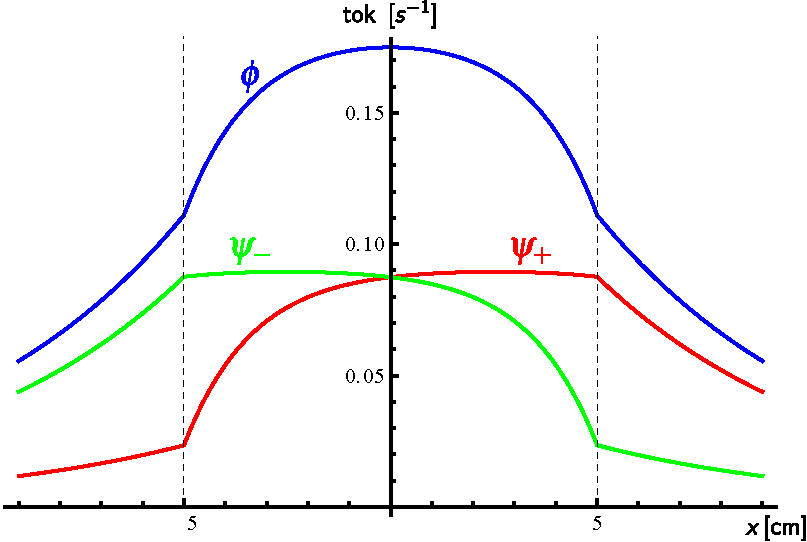
\includegraphics[height=.8\paperheight]{obr/doleva_doprava/distribuovany_075_05}

\end{frame}

\begin{frame}
  \frametitle{Příklad 1 -- v prostoru rozložený izotropní zdroj}
  \framesubtitle{$\bar\mu_{01} = 0$ (izotropní rozptyl)~~~~$\bar\mu_{02} = 0.5$}
  
  \centering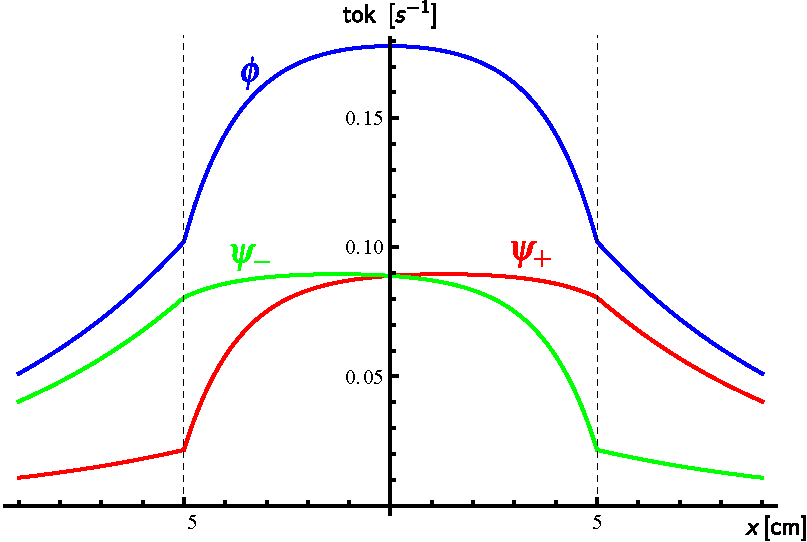
\includegraphics[height=.8\paperheight]{obr/doleva_doprava/distribuovany_0_05}

\end{frame}

\begin{frame}
  \frametitle{Příklad 1 -- v prostoru rozložený izotropní zdroj}
  \framesubtitle{$\bar\mu_{01} = 1$ (bez rozptylu)~~~~$\bar\mu_{02} = 0.5$}
  
  \centering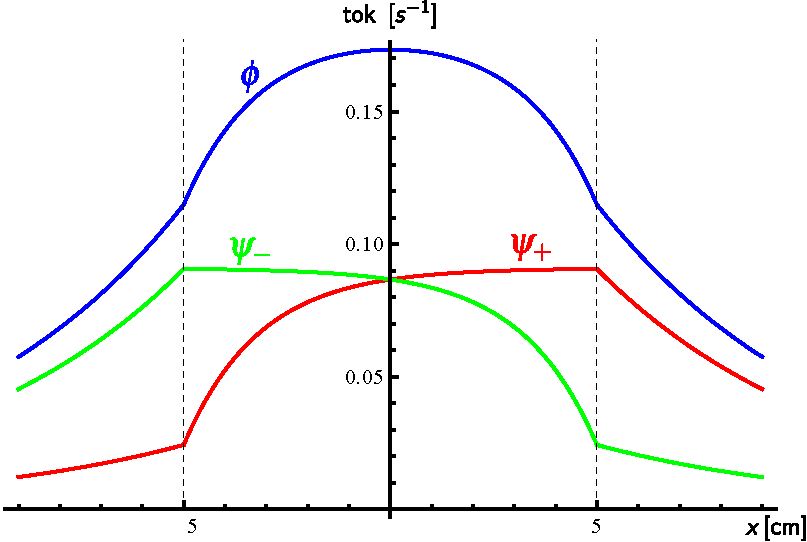
\includegraphics[height=.8\paperheight]{obr/doleva_doprava/distribuovany_1_05}

\end{frame}

\begin{frame}
  \frametitle{Příklad 1 -- v prostoru rozložený izotropní zdroj}
  \framesubtitle{$\bar\mu_{01} = 0.75$~~~~$\bar\mu_{02} = 1$ (bez rozptylu)}
  
  \centering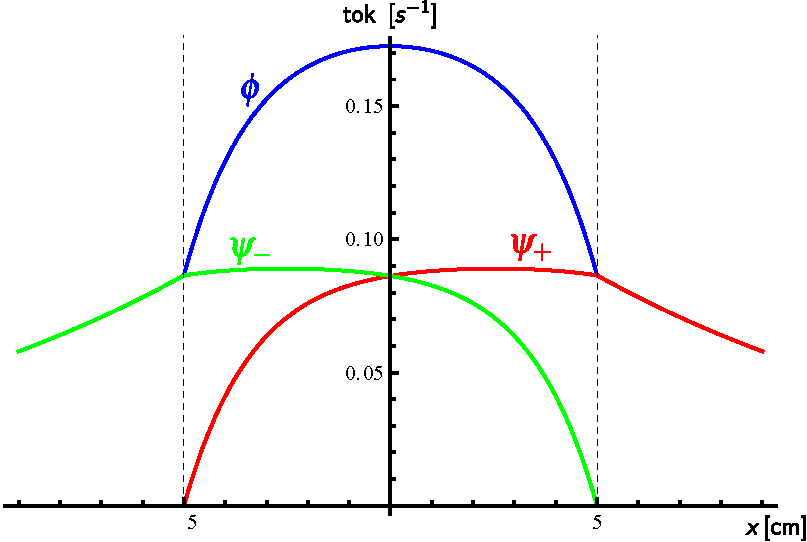
\includegraphics[height=.8\paperheight]{obr/doleva_doprava/distribuovany_075_1}

\end{frame}

\begin{frame}
  \frametitle{Příklad 1 -- v prostoru rozložený izotropní zdroj}
  \framesubtitle{$\bar\mu_{01} = 1$ (bez rozptylu)~~~~$\bar\mu_{02} = 1$ (bez rozptylu)}
  
  \centering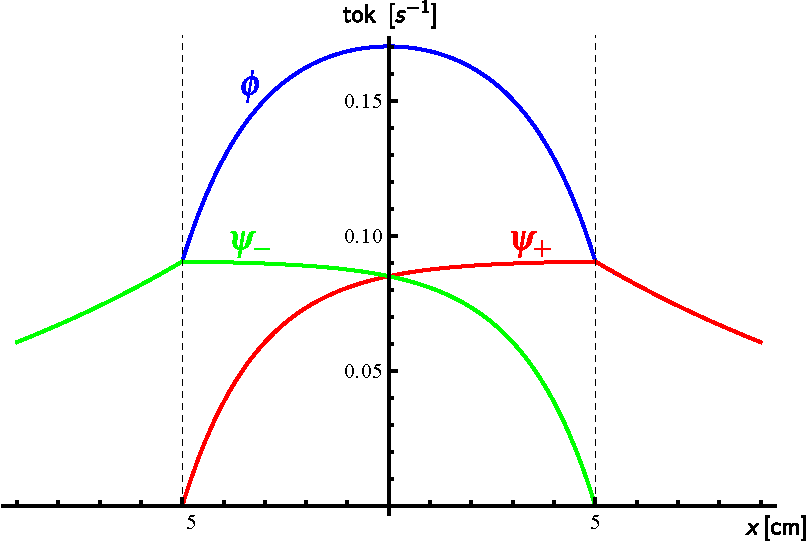
\includegraphics[height=.8\paperheight]{obr/doleva_doprava/distribuovany_1_1}

\end{frame}

\begin{frame}
  \frametitle{Příklad 2 -- bodový anizotropní zdroj}
  \framesubtitle{Data}
  
  \centering $\VV = (0,a)$~ ve vakuu\\
  
  \begin{myitemize}
  	\item $a = 5$\,cm
  	\item $\Sigma_t = 1$\,cm$^{-1}$,~ $\Sigma_a = 0.5$\,cm$^{-1}$
  	\item $S_+ = 0.7$\,s$^{-1}$,~ $S_- = 0.3$\,s$^{-1}$\\[.5em]
  	      $Q_\pm(x) = S_\pm\delta(x-x_Q)$ [cm$^{-1}$s$^{-1}$]\\[.5em]
  	      $x_Q=2$\,cm
  	\item $\muav = \textcolor<2>{blue}{\bar\mu_{01}}$
  \end{myitemize}


\end{frame}

\begin{frame}
  \frametitle{Příklad 2 -- bodový anizotropní zdroj}
  \framesubtitle{$\bar\mu_{01} = 0.75$}
  
  \centering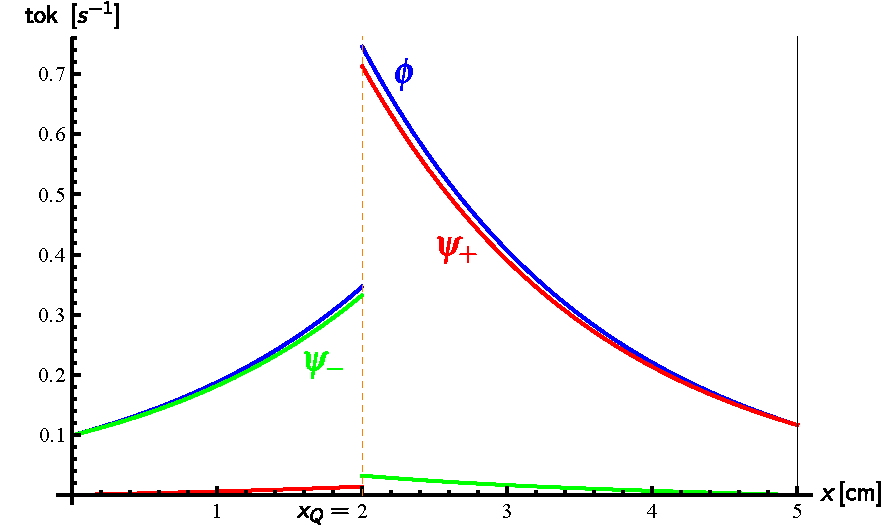
\includegraphics[height=.75\paperheight]{obr/doleva_doprava/bodovy_075}

\end{frame}

\begin{frame}
  \frametitle{Příklad 2 -- bodový anizotropní zdroj}
  \framesubtitle{$\bar\mu_{01} = 0$ (izotropní rozptyl)}
  
  \centering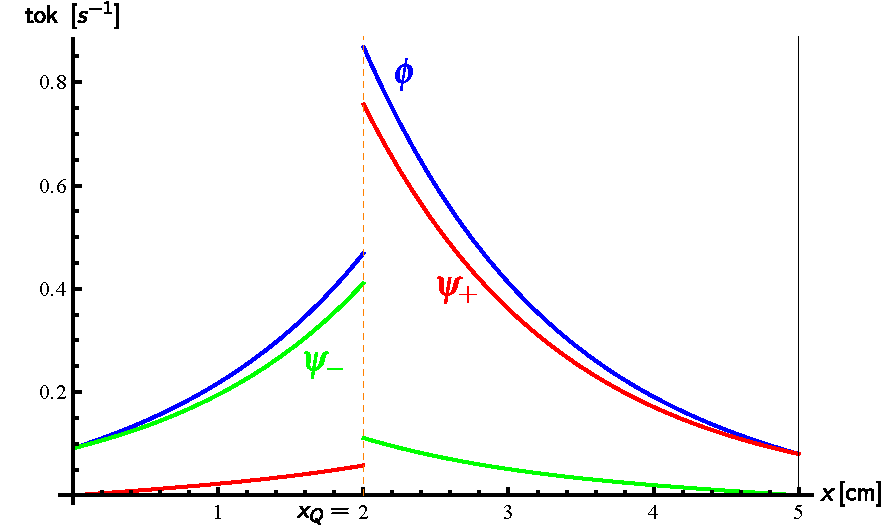
\includegraphics[height=.75\paperheight]{obr/doleva_doprava/bodovy_0}

\end{frame}

\begin{frame}
  \frametitle{Příklad 2 -- bodový anizotropní zdroj}
  \framesubtitle{$\bar\mu_{01} = 1$ (bez rozptylu)}
  
  \centering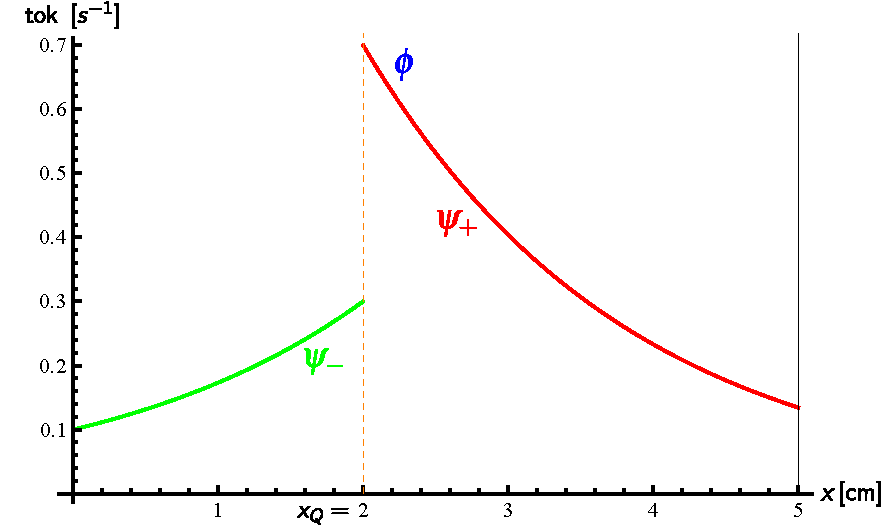
\includegraphics[height=.75\paperheight]{obr/doleva_doprava/bodovy_1}

\end{frame}

%\begin{frame}
%  \frametitle{Příklad -- v prostoru rozložený anizotropní zdroj}
%  \framesubtitle{Popis a tvar řešení}
%
%
%\end{frame}
%
%\begin{frame}
%  \frametitle{Příklad -- v prostoru rozložený anizotropní zdroj}
%  \framesubtitle{Průběh neutronových toků}
%
%
%\end{frame}
